
\documentclass[MAIN.tex]{subfiles} 
\begin{document} 
	%============================================================================ %

%======================================================================================== %
\begin{frame}
	\frametitle{Extreme Value Theory}
	\begin{itemize}
		\item The Extreme Value Theory (EVT) is extensively used for modelling very large and/or very small events. 
		\item Usually the focus of the analysis is the estimation of very extreme quantiles or tail probabilities. 
		\item It is widely used in several areas, such as environment, insurance, weather and hydrology. 
		\item Extreme value theory is important for assessing risk for highly unusual events, such as 100-year floods.
		\item Several R packages have been developed for fitting models in this framework. 
	\end{itemize}
	%This course aims to present the most common statistical tools of the EVT, as well as teaching the use of a R package.
\end{frame}

%======================================================================= %
%----------------------------------------------------------------------------------------%
\begin{frame}
\frametitle{Extreme Value Theory}

\begin{itemize}
\item The field of extreme value theory was pioneered by Leonard Tippett ($1902-1985$). 
\item Tippett was employed by the British Cotton Industry Research Association, where he worked to make cotton thread stronger. In his studies, he realized that the strength of a thread was controlled by the strength of its weakest fibers.

\item With the help of R. A. Fisher, Tippet obtained three asymptotic limits describing the distributions of extremes. The German mathematician Emil Julius Gumbel codified this theory in his 1958 book \textbf{\emph{Statistics of Extremes}}, including the Gumbel distributions that bear his name.
\end{itemize}
\end{frame}
%----------------------------------------------------------------------------------------%
\begin{frame}
%\frametitle{EVT: Frequency Analysis}
%%---http://ihpnagoyaforum.org/textbooks/TakaraLecture.pdf
%%----------------------------------------------------------------------------------------%
%\begin{itemize}
%	\item Frequency Analysis ($FA$): Probabilistic description of hydrological extremes
%	\item Extraction of extreme variables from data
%	\item Choice of a distribution
%	\item Parameter estimation
%	\item Quantiles + uncertainty
%\end{itemize}
\begin{figure}
\centering
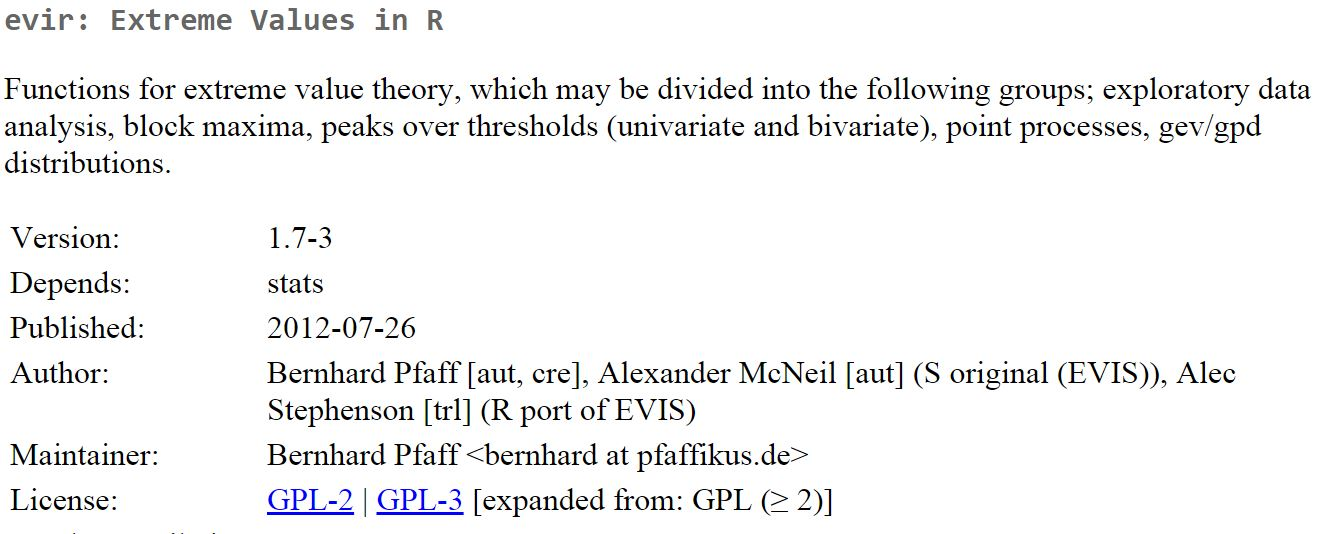
\includegraphics[width=1.05\linewidth]{images/evir}

\end{figure}

\end{frame}


%%======================================================================================== %
%\begin{frame}
%	\frametitle{Extreme Value Distribution} Extreme Value. The extreme value distribution is often used to model extreme events, such as the size of floods, gust velocities encountered by airplanes, maxima of stock market indices over a given year, etc.; it is also often used in reliability testing, for example in order to represent the distribution of failure times for electric circuits (see Hahn and Shapiro, 1967). The extreme value (Type I) distribution has the probability density function:
%	
%	\[f(x) = 1/b \times e^{[-(x-a)/b]} \times e^{-e^{[-(x-a)/b]}},    for -8 < x < 8, b > 0\]
%	
%	where
%	
%	a	is the location parameter
%	b	is the scale parameter
%	e	is the base of the natural logarithm, sometimes called Euler's e (2.71...)
%\end{frame}
\end{document}